\documentclass{article}
\usepackage[utf8]{inputenc}
\usepackage{geometry}
\usepackage{listings}
\usepackage{graphicx}
\usepackage{subcaption}
\usepackage{titling}
\usepackage{fancyhdr}
\usepackage{lipsum}
\usepackage{cmbright}

\geometry{
    a4paper,
    total={170mm,257mm},
    left=20mm,
    top=20mm,
}

\title{\textbf{Operating Systems Assignment}\\
(Implementation of \textbf{Banker's Algorithm} for Deadlock Avoidance)
}
\author{Akhil Katlagunta}
\date{April 2025}

\fancypagestyle{plain}{%
    \fancyhf{} % clear all header and footer fields
    \fancyfoot[R]{\thepage}
    \fancyfoot[L]{\thedate}
    \fancyhead[L]{Operating System Assignment}
    \fancyhead[R]{\theauthor}
}

\makeatletter
\def\@maketitle{%
  \newpage
  \noindent\begin{tabular}{@{}ll}
    \textbf{Name:} & \theauthor\\
    \textbf{Roll Number:} & % your roll number\\
    \textbf{Division:} & % your class\\
    \textbf{Enrollment Number:} & % your enrollment number
  \end{tabular}
  \null
  \vskip 2em%
  \begin{center}%
    \let \footnote \thanks
    {\LARGE \@title \par}%
    \vskip 1em%
  \end{center}%
  \par
  \vskip 1em}
\makeatother

\pagestyle{plain}

\begin{document}

\maketitle

\noindent\rule{\textwidth}{0.4pt}

\section*{Theory}
The Banker's Algorithm is a deadlock avoidance algorithm used in operating systems. It is named so because it compares the resource allocation problem to a bank loaning money such that it never allocates funds in a way that could lead to unsafe states (where all funds may not be returned).

\vspace{1em}
The algorithm uses three main matrices:

\begin{itemize}
    \item \textbf{Allocation Matrix:} The current allocation of each resource type to each process.
    \item \textbf{Maximum Demand Matrix:} The maximum number of each resource that each process may request.
    \item \textbf{Available Vector:} The number of available instances for each resource type.
\end{itemize}

\noindent From these, a Need Matrix is calculated:

\begin{lstlisting}[language=Python]
Need[i][j] = Max[i][j] - Allocation[i][j]
\end{lstlisting}

\noindent\rule{\textwidth}{0.4pt}

\section*{Procedure}
The algorithm works as follows:

\begin{enumerate}
    \item It checks if there is a safe sequence in which all processes can complete.
    \item A process is said to be safely executable if its needs can be satisfied with the currently available resources.
    \item If such a process is found, it is assumed to execute and release its resources, which are added back to the available pool.
    \item This continues until all processes can complete, proving the system is in a safe state.
\end{enumerate}

\noindent If no such sequence exists, the system is in an unsafe state, which may lead to deadlock.

\vspace{15pt}
\noindent\rule{\textwidth}{0.4pt}

\newpage

\section*{Screenshots}

\begin{figure}[h!]
    \centering
    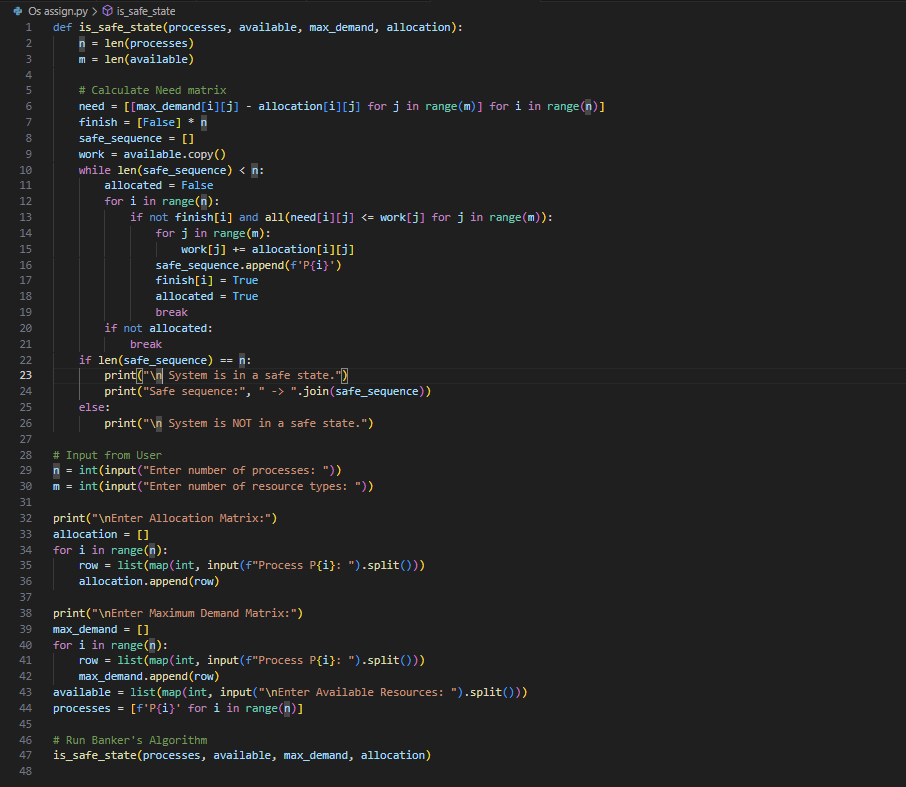
\includegraphics[width=0.8\textwidth]{1.png}
    \caption{Input of Banker's Algorithm Simulation}
    \label{fig:bankeroutput}
\end{figure}

\begin{figure}[h!]
    \centering
    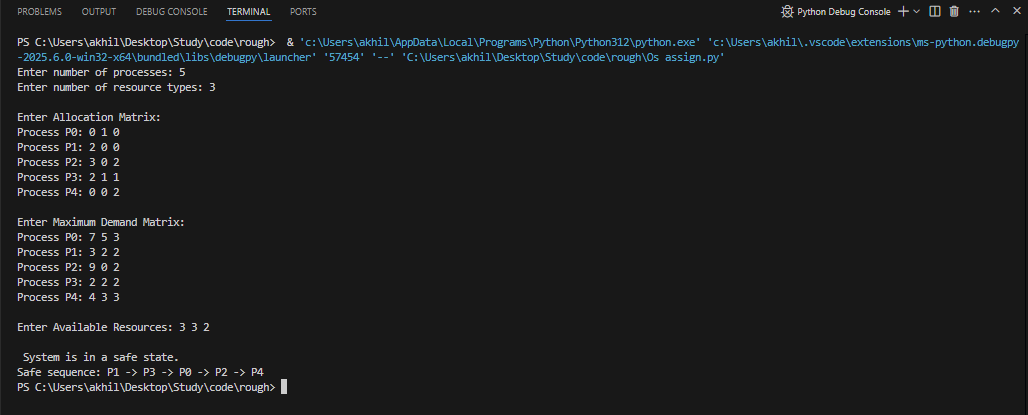
\includegraphics[width=1\textwidth]{2.png}
    \caption{Output of Banker's Algorithm Simulation}
    \label{fig:bankeroutput}
\end{figure}

\end{document}
